\documentclass[journal,12pt,twocolumn]{IEEEtran}
%
\usepackage{setspace}
\usepackage{gensymb}
%\doublespacing
\singlespacing

\usepackage[cmex10]{amsmath}
\usepackage{amsthm}
%\usepackage{iithtlc}
\usepackage{mathrsfs}
\usepackage{txfonts}
\usepackage{stfloats}
\usepackage{bm}
\usepackage{cite}
\usepackage{cases}
\usepackage{subfig}
%\usepackage{xtab}
\usepackage{longtable}
\usepackage{multirow}
%\usepackage{algorithm}
%\usepackage{algpseudocode}
\usepackage{enumitem}
\usepackage{mathtools}
\usepackage{steinmetz}
\usepackage{tikz}
\usepackage{circuitikz}
\usepackage{verbatim}
\usepackage{tfrupee}
\usepackage[breaklinks=true]{hyperref}
%\usepackage{stmaryrd}
\usepackage{tkz-euclide} % loads  TikZ and tkz-base
%\usetkzobj{all}
\usetikzlibrary{calc,math}
\usepackage{listings}
    \usepackage{color}                                            %%
    \usepackage{array}                                            %%
    \usepackage{longtable}                                        %%
    \usepackage{calc}                                             %%
    \usepackage{multirow}                                         %%
    \usepackage{hhline}                                           %%
    \usepackage{ifthen}                                           %%
  %optionally (for landscape tables embedded in another document): %%
    \usepackage{lscape}     
\usepackage{multicol}
\usepackage{chngcntr}
%\usepackage{enumerate}

%\usepackage{wasysym}
%\newcounter{MYtempeqncnt}
\DeclareMathOperator*{\Res}{Res}
%\renewcommand{\baselinestretch}{2}
\renewcommand\thesection{\arabic{section}}
\renewcommand\thesubsection{\thesection.\arabic{subsection}}
\renewcommand\thesubsubsection{\thesubsection.\arabic{subsubsection}}

\renewcommand\thesectiondis{\arabic{section}}
\renewcommand\thesubsectiondis{\thesectiondis.\arabic{subsection}}
\renewcommand\thesubsubsectiondis{\thesubsectiondis.\arabic{subsubsection}}

% correct bad hyphenation here
\hyphenation{op-tical net-works semi-conduc-tor}
\def\inputGnumericTable{}                                 %%

\lstset{
%language=C,
frame=single, 
breaklines=true,
columns=fullflexible
}
\newenvironment{amatrix}[1]{%
  \left(\begin{array}{@{}*{#1}{c}|c@{}}
}{%
  \end{array}\right)
}
\DeclarePairedDelimiter\abs{\lvert}{\rvert}%
\DeclarePairedDelimiter\norm{\lVert}{\rVert}%

% Swap the definition of \abs* and \norm*, so that \abs
% and \norm resizes the size of the brackets, and the 
% starred version does not.
\makeatletter
\let\oldabs\abs
\def\abs{\@ifstar{\oldabs}{\oldabs*}}
%
\let\oldnorm\norm
\def\norm{\@ifstar{\oldnorm}{\oldnorm*}}
\makeatother

\newtheorem{theorem}{Theorem}[section]
\newtheorem{problem}{Problem}
\newtheorem{proposition}{Proposition}[section]
\newtheorem{lemma}{Lemma}[section]
\newtheorem{corollary}[theorem]{Corollary}
\newtheorem{example}{Example}[section]
\newtheorem{definition}[problem]{Definition}
%\newtheorem{thm}{Theorem}[section] 
%\newtheorem{defn}[thm]{Definition}
%\newtheorem{algorithm}{Algorithm}[section]
%\newtheorem{cor}{Corollary}
\newcommand{\BEQA}{\begin{eqnarray}}
\newcommand{\EEQA}{\end{eqnarray}}
\newcommand{\define}{\stackrel{\triangle}{=}}
\bibliographystyle{IEEEtran}
%\bibliographystyle{ieeetr}
\providecommand{\mbf}{\mathbf}
\providecommand{\pr}[1]{\ensuremath{\Pr\left(#1\right)}}
\providecommand{\qfunc}[1]{\ensuremath{Q\left(#1\right)}}
\providecommand{\sbrak}[1]{\ensuremath{{}\left[#1\right]}}
\providecommand{\lsbrak}[1]{\ensuremath{{}\left[#1\right.}}
\providecommand{\rsbrak}[1]{\ensuremath{{}\left.#1\right]}}
\providecommand{\brak}[1]{\ensuremath{\left(#1\right)}}
\providecommand{\lbrak}[1]{\ensuremath{\left(#1\right.}}
\providecommand{\rbrak}[1]{\ensuremath{\left.#1\right)}}
\providecommand{\cbrak}[1]{\ensuremath{\left\{#1\right\}}}
\providecommand{\lcbrak}[1]{\ensuremath{\left\{#1\right.}}
\providecommand{\rcbrak}[1]{\ensuremath{\left.#1\right\}}}

\providecommand{\system}{\overset{\mathcal{H}}{ \longleftrightarrow}}
	%\newcommand{\solution}[2]{\textbf{Solution:}{#1}}
\newcommand{\solution}{\noindent \textbf{Solution: }}
\newcommand{\cosec}{\,\text{cosec}\,}
\providecommand{\dec}[2]{\ensuremath{\overset{#1}{\underset{#2}{\gtrless}}}}
\newcommand{\myvec}[1]{\ensuremath{\begin{pmatrix}#1\end{pmatrix}}}
\newcommand{\mydet}[1]{\ensuremath{\begin{vmatrix}#1\end{vmatrix}}}
%\numberwithin{equation}{section}
\numberwithin{equation}{subsection}
%\numberwithin{problem}{section}
%\numberwithin{definition}{section}
\makeatletter
\@addtoreset{figure}{problem}
\makeatother
\let\StandardTheFigure\thefigure
\let\vec\mathbf


\begin{document}

\begin{center}
\huge Assignment 2

\large Shaik Zeeshan Ali\\
AI20MTECH11001
\end{center}
\begin{abstract}
This document explains how to find the shortest distance between two lines if and when the two lines are not intersecting with each other.
\end{abstract}
Download all python codes from 
\begin{lstlisting}
https://github.com/Zeeshan-IITH/IITH-EE5609/new/master/codes
\end{lstlisting}

and latex-tikz codes from 
\begin{lstlisting}
https://github.com/Zeeshan-IITH/IITH-EE5609
\end{lstlisting}

\section{Problem}
Find the shortest distance between the lines 
\begin{align}
    L_1\colon \vec{x}=\myvec{1\\2\\1}+\lambda_1\myvec{1\\-1\\1}\\
    L_2\colon \vec{x}=\myvec{2\\-1\\-1}+\lambda_2\myvec{2\\1\\2}
\end{align}
\section{construction}
When two lines are not intersecting the distance between them is non-zero.The equation of above mentioned lines in symmetric form is
\begin{align}
    L_1\colon x-1=2-y=z-1\\
    L_2\colon \frac{x-2}{2}=y+1=\frac{z+1}{2}
\end{align}
The above line equations have no point of intersection as for no value of $\lambda_1,\lambda_2$ both the equations (2.0.1) and (2.0.2) are equal.\par
If the two line intersect then (2.0.1)=(2.0.2) i.e.
\begin{align}
    \myvec{1\\2\\1}+\lambda_1\myvec{1\\-1\\1}=\myvec{2\\-1\\-1}+\lambda_2\myvec{2\\1\\2}\\
    \lambda_1\myvec{1\\-1\\1}-\lambda_2\myvec{2\\1\\2}=\myvec{1\\-3\\-2}\\
    \myvec{1 & -2\\-1 & -1\\1 & -2}\myvec{\lambda_1\\\lambda_2}=\myvec{1\\-3\\-2}\\
    \intertext{The Augmented matrix will be}
    \myvec{1 & -2 & 1\\-1 & -1 & -3\\1 & -2 & -2}\\
    \myvec{1 & -2 & 1\\-1 & -1 & -3\\1 & -2 & -2}\xleftrightarrow{R_1=R_1-R_2}\myvec{0 & 0 & 3\\-1 & -1 & -3\\1 & -2 & -2}
\end{align}
The above matrix has a $rank=3$ .Hence the lines do not intersect.
\section{solution}
Let $A$ be a point on line $L_1$ and $B$ be point on the line $L_2$.Then the shortest distance between two skew lines will be the length of line perpendicular to both the lines $L_1$,$L_2$ and passing through $A$ and $B$.\par
The vector passing through the points $A$ and $B$ will be
\begin{align}
    \vec{A-B}=\vec{x_1-x_2}+\myvec{\vec{m_1} & -\vec{m_2}}\myvec{\lambda_1\\\lambda_2}
\end{align}
The vectors $\vec{m_1}$,$\vec{m_2}$ are both perpendicular to the line ${AB}$.So the dot product of $\vec{m_1}$,$\vec{m_2}$ with the line ${AB}$ is zero.\par
The dot product of $\vec{m_1}$ with the line ${AB}$ is
\begin{align}
    \vec{m_1}^T\brak{\vec{A-B}}=0\\
    \vec{m_1^T}(\vec{x_1-x_2})+\vec{m_1^T}(\vec{m_1} & -\vec{m_2})\begin{pmatrix}\lambda_1 \\ \lambda_2\end{pmatrix}=0
\end{align}
The dot product of $\vec{m_2}$ with the line ${AB}$ is
\begin{align}
    \vec{m_2}^T\brak{\vec{A-B}}=0\\
    \vec{m_1^T}(\vec{x_1-x_2})+\vec{m_2^T}(\vec{m_1} & -\vec{m_2})\myvec{\lambda_1 \\ \lambda_2}=0
\end{align}
Let the matrix $\vec{M}$ be
\begin{align}
    \vec{M}=\myvec{\vec{m_1}^T\\\vec{m_2}^T}
\end{align}
Combining the equations $(3.0.3)$ and $(3.0.5)$ in matrix form,using equation $(3.0.6)$, we get
\begin{align}
    \vec{M}\vec{M}^T\myvec{\lambda_1\\-\lambda_2}+\vec{M}\vec{(x_1-x_2)}=0
\end{align}
simplifying it further
\begin{align}
    \vec{M}\vec{M}^T\begin{pmatrix}\lambda_1\\-\lambda_2\end{pmatrix}=\vec{M}\vec{(x_2-x_1)}
\end{align}
To find the points on the lines which make up the shortest distance we need to find $\lambda_1$ and $\lambda_2$ using the above expression to get the augmented form
\begin{align}
    \myvec{\vec{m_1}^T\vec{m_1} & \vec{m_1}^T\vec{m_2}\\\vec{m_2}^T\vec{m_1} & \vec{m_2}^T\vec{m_2}}\myvec{\lambda_1\\-\lambda_2}=\myvec{\vec{m_1}^T\vec{(x_2-x_1)}\\\vec{m_2}^T\vec{(x_2-x_1)}}\\
    \myvec{\vec{m_1}^T\vec{m_1} & \vec{m_1}^T\vec{m_2} & \vec{m_1}^T\vec{(x_2-x_1)}\\\vec{m_2}^T\vec{m_1} & \vec{m_2}^T\vec{m_2} & \vec{m_2}^T\vec{(x_2-x_1)}}\\
    \intertext{we know that}
    \vec{x_1}=\myvec{1\\2\\1},\vec{x_2}=\myvec{2\\-1\\-1},\vec{m_1}=\myvec{1\\-1\\1} and  \vec{m_2}=\myvec{2\\1\\2}\notag
    \intertext{so the augmented matrix will be}
    \myvec{{2}3 & 3 &2\\ 3 & 9 & -5}
    \intertext{Using row reduction method to get row-reduced echelon form, we get}
    \myvec{23 & 3 &2\\ 3 & 9 & -5}\xleftrightarrow{R_2=R_2-R_1}\myvec{3 & 3 &2\\ 0 & 6 & -7}\\
    \myvec{3 & 3 &2\\ 0 & 6 & -7}\xleftrightarrow{R_1=2R_1-R_2}\myvec{6 & 0 & 11\\ 0 & 6 & -7}\\
    \intertext{scaling with $6$,we get}
    \myvec{6 & 0 & 11\\ 0 & 6 & -7}\xleftrightarrow{R_1=\frac{R_1}{6},R_2=\frac{R_2}{6}}\myvec{1 & 0 & \frac{11}{6}\\ 0 & 1 & \frac{-7}{6}}
\end{align}
So the values are $\lambda_1=\frac{11}{6}$ and $\lambda_2=\frac{7}{6}$.
Using the equation (1.0.1) and (1.0.2), we get the points as $\frac{1}{6}\myvec{17\\1\\17}$ and $\frac{1}{6}\myvec{26\\1\\8}$ on the line $L_1$,$L_2$ respectively.\par
The shortest distance between the lines is the distance between the points $A$ and $B$.
\begin{equation}
    \norm{(\vec{B}-\vec{A})}\\
    =\norm{\frac{1}{{6}}\myvec{17\\1\\17}-\frac{1}{{6}}\myvec{26\\1\\8}}\\
    =\frac{3}{\sqrt{2}}
\end{equation}
Therefore the shortest distance between the given lines is $\frac{3}{\sqrt{2}}$.\par

The unit vector perpendicular to lines
\begin{align}
    Line_1\colon \vec{x}=\vec{x_1}+\lambda_1\vec{m_1}\\
    Line_2\colon \vec{x}=\vec{x_2}+\lambda_1\vec{m_2}
\end{align}
can be found by 
\begin{align}
    \frac{\vec{A-B}}{\norm{\vec{A-B}}}\\
    \frac{\frac{1}{{6}}\myvec{17\\1\\17}-\frac{1}{{6}}\myvec{26\\1\\8}}{\frac{3}{\sqrt{2}}}\notag
\end{align}

So the unit vector perpendicular to both $L_1$ and $L_2$ is
\begin{align}
    \vec{n}=\frac{1}{\sqrt{2}}\begin{pmatrix}-1\\0\\1\end{pmatrix}
\end{align}
\begin{figure}[!]
\begin{center}
    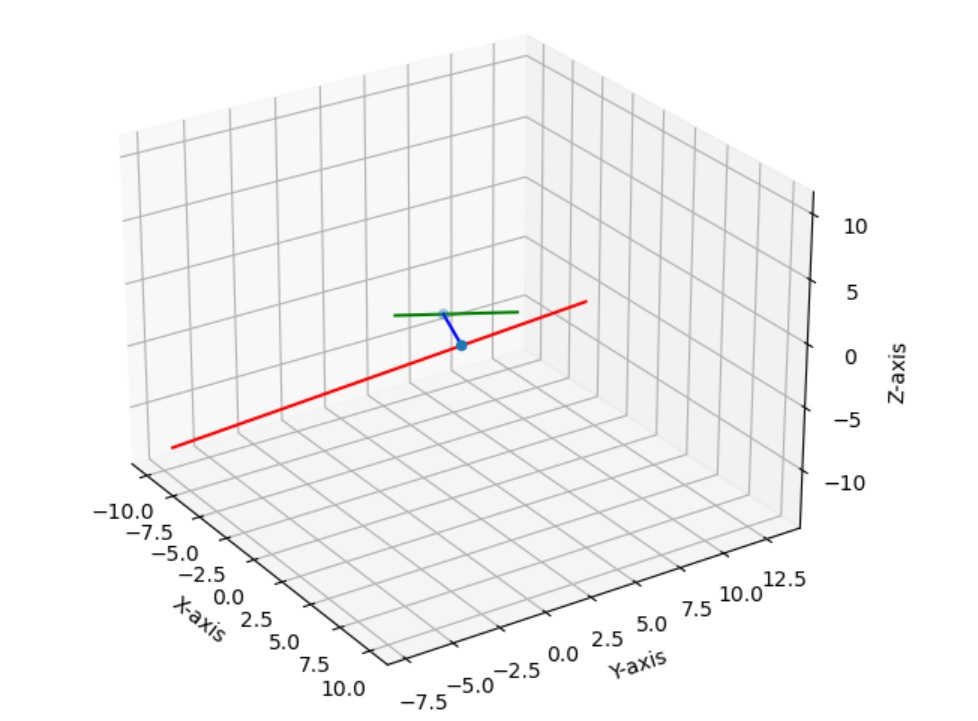
\includegraphics[width=11cm]{assignment2.jpg}
    \caption{This is the plot of the given skew lines and the blue line indicates the normal to the given lines}
    \label{Skew_lines}
\end{center}
\end{figure}
\end{document}
